\documentclass[10pt]{sensys-proc}
%\usepackage{titling}
%\setlength{\droptitle}{-10em}

\usepackage{graphicx}
\usepackage{balance}
\usepackage{comment}
\usepackage{tabularx}
\usepackage{amssymb}
\usepackage{amsmath}

\numberofauthors{1}

\author{
\alignauthor Gabe Fierro, Omar Rehmane, Andrew Krioukov, David Culler\\
       \affaddr{Computer Science Department}\\
       \affaddr{University of California, Berkeley}\\
       \affaddr{ gt.fierro@berkeley.edu, orehmane@berkeley.edu,\\krioukov@cs.berkeley.edu, culler@cs.berkeley.edu}
}

\title{Demo Abstract: Zone-level Occupancy Counting with Existing Infrastructure} 

\crdata{978-1-4503-1170-0}
\conferenceinfo{Buildsys'12,} {November 6, 2012, Toronto, ON, Canada.}
\CopyrightYear{2012}

\begin{document}

\maketitle

\section{Introduction}

Obtaining real-time counts of occupants in each room/zone within a building has been one of the holy grails of building automation. Occupancy counts can be used as an input to a wide range of controls in buildings, drastically improving energy efficiency. For example,  ventilation can be set in proportion to occupancy, air conditioning can be disabled or turned down for empty or sparsely populated areas, lights can be unobtrusively turned on/off without waving at a motion detector and plug-loads in empty areas can be monitored or turned off. These techniques can make a building's energy consumption proportional to the number of people in the space, whereas today most buildings operate wastefully in just two static modes: fully occupied or unoccupied. For buildings that are never completely empty, such as labs and graduate student offices, this static regime requires that the building continue to operate at night almost the same as during the day.

The major challenge is to obtain counts of occupants cheaply, reliably, and without requiring any new actions from occupants. Previous efforts have used motion detectors (PIR) with reed switches~\cite{Agarwal2010, Lu2010}, infrared (IR) beams~\cite{sun9}, video cameras~\cite{Erickson11}, RFID tags, thermal imaging and $CO_2$ sensors. All of these approaches require the deployment of new hardware, hampering scalability, and vary in their accuracy and granularity. Motion detectors can only detect the presence of people, not their number. $CO_2$ sensors approximate the number of people in an enclosed space, but cannot granularly count people in cubicle areas. IR beams are cheap and accurate but must be placed at all entrances and exits to an area. RFID requires occupants to carry special tags and requires large readers to be placed at all entrances. 

Observing that most building occupants on campus regularly carry smartphones and other wireless devices, we explore people-counting using just existing infrastructure. Our guiding design principles are that no new actions should be required of occupants, counts are required with coarse, zone-level granularity (e.g. lighting zones as shown in Figure~\ref{fig:floormap}), and deployment time and hardware requirements should be minimized.

We apply a {\it passive localization} technique used in the wireless networking literature for rogue access point detection~\cite{Faria2006, Laurendeau2010} to locate and count occupants by their mobile devices. With this technique 802.11 wireless infrastructure is used to overhear packets sent by client devices and to measure the received signal strength (RSSI). Thus, occupants can be counted without a special phone application; we only require that WiFi is enabled on the phone and and automatically associated with any wireless network. On our test Android and iPhone devices this happens automatically even when the phone's screen is turned off and without the user pressing any buttons. Since only zone-level precision is required, we can effectively solve a classification problem ({\it i.e. which zone is a phone in?}) instead of a general localization problem. This significantly reduces error and allows us to use a localization algorithm that requires no training. Compared to prior work on indoor wireless localization, we focus on coarse-grained and completely passive localization tailored for counting occupants in buildings.

%captive portal, only upload matters





%Our localization infrastructure differs from that of previous work in that it is not focused on precision, but rather tuned towards the application of loose-grained occupancy detection for the purpose of localized building actuation. By accurately determining the number of occupants in each of a series of predefined zones, we can adjust the lighting and heating in each zone appropriately, our infrastructure need only fulfill the level of granularity provided by the building actuation controls.

%While there are multiple ways to obtain that zone-level count, they hold other drawbacks and challenges.  Motion detectors provide no way for the user to set settings, and make getting a reliable per-zone count difficult.  As for RFID-equipped cards, those are expensive and require deployment of specialized equipment.  By contrast, this approach leverages existing deployed infrastructure and technology, minimizing cost and difficulty of deployment while achieving a high level of efficacy.

%A large body of previous work done in the area of localization relies on specialized hardware, dense hardware placement, generous sets of training data, or a combination thereof. The ubiquitous nature of 802.11 wireless networks presents an opportunity for leveraging existing wireless infrastructure with the addition of a small number of cheap and widely available devices to create a localization solution that does not require training data, instead relying on robust algorithms to make use of existing data.

%\begin{itemize}
%\item talk about advantages of passive localization over active localization -- if we don't require the occupants to do much, then we don't have to rely on them for accuracy
%\item mention some of the previous work here
%\item maybe talk about with BAS, we can easily incorporate the infrastructure with our pre-built actuation stuff
%\end{itemize}
\section{Infrastructure}
Our infrastructure utilizes routers each installed with OpenWRT -- a free Linux-based router firmware -- running a cross-compiled version of tcpdump.  Specifically, our setup consisted of Buffalo AG300H routers, though any router with an omnidirectional antenna would serve adequately. The property that this infrastructure uses only free and open-source software and cheap, widely-available hardware differentiates it in the arenas of plausibility and realistic deployment from previous work that uses complicated, obscure, and/or special purpose (albeit possibly cheap) hardware. 

\begin{figure}[htb]
\begin{center}
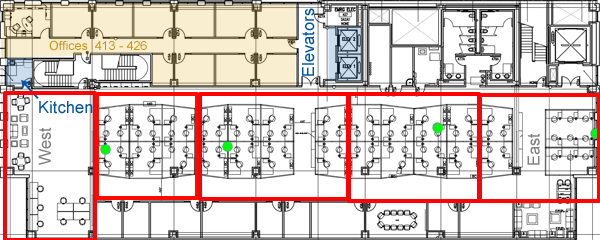
\includegraphics[width=\linewidth]{figs/floor4}
\end{center}
\caption{Location of routers (green) shown in relation to actuation zones (red). Note we do not need to place the routers in a convex hull of the entire floor in order to place a user within a zone.}
\end{figure}

The campus network on which we chose to deploy was a 2.4Ghz wireless network supporting channels 1, 6, and 11. Each of the routers was set to \emph{monitor/promiscuous} mode, and was installed with tcpdump-4.2.1, an open-source packet analyzer. Because routers typically lack the processing power and memory for processing large amounts of data, we connected our routers to a central computer (a FitPC running Ubuntu Linux). The manner of the connection between routers and central computer can be through a wired network or through direct Ethernet. It is the job of this central computer to mitigate the collection of packet data from each of the routers, perform the necessary mathematical operations, and process the results against a list of known MAC addresses. 

The routers cycle through each of the three wireless channels using tcpdump-4.2.1 to capture packets in 1-second increments. Each packet is forwarded along with its 802.11 radiotap link-level header over SSH to the central computer, which parses out the RSSI and source MAC address. For recognized MAC addresses, for each time-step for a given sample rate, each RSSI is converted to a linear scale and the resulting RSSIs are averaged per router. We can then compute the possible location $(x_d,y_d)$ of the device possessing a given MAC address as the centroid of the known router coordinates $(x_i, y_i)$ weighted by the average detected signal strength at that router $r_i$:
\begin{equation}
\begin{split}
x_d, y_d = \displaystyle\sum_{i} \frac{r_ix_i, r_iy_i}{\displaystyle\sum_i r_i}
\end{split}
\end{equation}
The central computer stores the 10 most recent computed centroids, and the location of the device is computed as the average of the 5 most closely clustered centroids of the 10 cached centroids (using Manhattan Distance as a heuristic). In practice, this ``averaging of averages'' greatly reduces the influence of the deployment environment upon the consistency of the measured RSSIs. Abnormally strong or weak signals thus do not alter the accuracy of our estimations. There is an incurred lag of about 4 times the sample rate should the device move, but this delay is acceptable within the bounds of accurate occupancy detection. We are able to place devices within 1 cubicle of their actual location (about 10 feet). This grade of accuracy is lower than other trained systems such as X Y and Z, but because light banks and HVAC dampers cannot differentiate between two adjacent cubicles, our system need not as well.

The passive nature of our localization infrastructure means that it requires little, if any, effort on behalf of the occupants to perform. Once we know the MAC addresses for all wifi-enabled devices associated with a given user, we can obtain a session IP address for a device by listening to all wireless traffic. In the absence of regular or sufficient traffic, the central computer can occasionally ping the device in question to either elicit the requisite wireless traffic or determine if the device has left the tracking area (which suggests the user has left). This approach differs from previous wireless localization work in that it does not \emph{require} the user to ensure he/she is creating enough traffic to be localized accurately, but rather unobtrusively generates the necessary data. 

This raises the issue of accounting for ``detached devices,'' devices left connected to the network that are not actively being used and can therefore be falsely registered as occupants. This can be ignored in the context of binary occupancy detection (``occupied'' versus ``not occupied''), but in applications requiring more exact counts, the problem of detached devices can be approached with analysis of the specific types of packets sent by the device in question. For example, if the device is sending DHCP authentication packets, we can assume the device may be associated with the given network but not logged-in, suggesting the device is not currently being used. Analysis of the number of HTTP packets for a given device can indicate the type and activity level of the device: low-frequency laptop traffic might suggest a detached device, whereas high-frequency mobile phone traffic implies an active user.

An additional strength of our infrastructure is the possibility for it to exist entirely on the incumbent router setup, e.g. by being installed as part of the proprietary Cisco router firmware. 

It is a simple matter to map arbitrary polygons to the areas affected by specific lightbanks or HVAC drivers, and thusly provide occupant-driven actuation. Systems such as BAS facilitate the actuation of a space based on geospatial coordinates.

In order to place an occupant within a space, it is necessary to have the routers form a convex hull of said space. However, because of the low granularity of building actuation controls, fewer routers may be used to 

\begin{figure}[htb]
\begin{center}
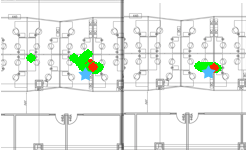
\includegraphics[width=.6\linewidth]{figs/samplesize}
\end{center}
\caption{increased accuracy with increasingly large sample rates (20s, left; 10s, right). Even at times of low ambient signal noise, weighted centroid measurements can be inconsistent (green), a problem remedied by averaging the 5 most closely clustered centroids (red).}
\end{figure}

\begin{itemize}
\item wireless localization tailored for buildings, passive is key. We reuse existing infrastructure (not entirely, actually, bec this is a prottype, but in real life we would get Cisco to do this on their routers)

\item need to elicit data from user phones

\item no need for training -- easily generalize

\item how easy this is to map into our current acutation setup

\item how is this better than existing solutions like RFID, motion sensors, laser gates, other wifi localization

\item include picture of setup of floor on SDH floor plan. Locations of routers, location of device, guessed centroids, 'averaged' centroids, etc

caption: increased accuracy with increasingly large sample rates. Even when measured at times of low ambient noise, measurements can be inconsistent (green/light grey), a problem remedied by averaging the 5 most closely clustered centroids (red/dark grey)

\item mac address and IPs, get traffic, pull out iP, generate traffic

\item how to detect stationary devices. We can do automatic detection, but if occupants abandon a device,  "detatched devices"

\end{itemize}

{
\scriptsize
\bibliographystyle{acm}
\bibliography{paper}
}
\end{document}


%Citations
%http://www.sun9powersaving.com/how-it-works.html
%Occupancy-Driven Energy Management for Smart Building Automation

